\chapter{Projectübersicht}

Die Firma { {{- project.customer -}} } beauftragte uns einen Penetrationstest für den Zeitraum
vom { {{- project.start_date|date('d.M.Y') -}} } bis { {{- project.end_date|date('d.M.Y') -}} } durchzuführen.
\\
Der Scope wurde wie folgt festgelegt:
\begin{itemize}
    
    \item {{ scope.name }}
    
\end{itemize}

Die Tabelle \ref{tbl:host-summary} zeigt eine Übersicht der Systeme, die während des Penetrationstests ermittelt werden konnten.

\begin{table}[ht]
    \renewcommand{\arraystretch}{1.5}
    \centering
    \begin{tabularx}{\textwidth}{| X | X | X |}
        \hline
        \textbf{Host} & \textbf{OS} & \textbf{Hostnames} \\
        \hline
        
        {{ host.ip }} & {{ host.os }} & {{ host.get_hostnames() }}    \\
        \hline
        
    \end{tabularx}
    \caption{Host Übersicht}
    \label{tbl:host-summary}
\end{table}


Als Resultat, wurden Schwachstellen in den untersuchten Systemen gefunden, welche ein erhöhtes Risiko darstellen.


Die Grafik \ref{fig:bsi} zeigt die Klassifikation eines Penetrationstests nach dem Standardmodell des Bundesamtes für Sicherheit in der Informationstechnik.

\begin{figure}[h]
\centering
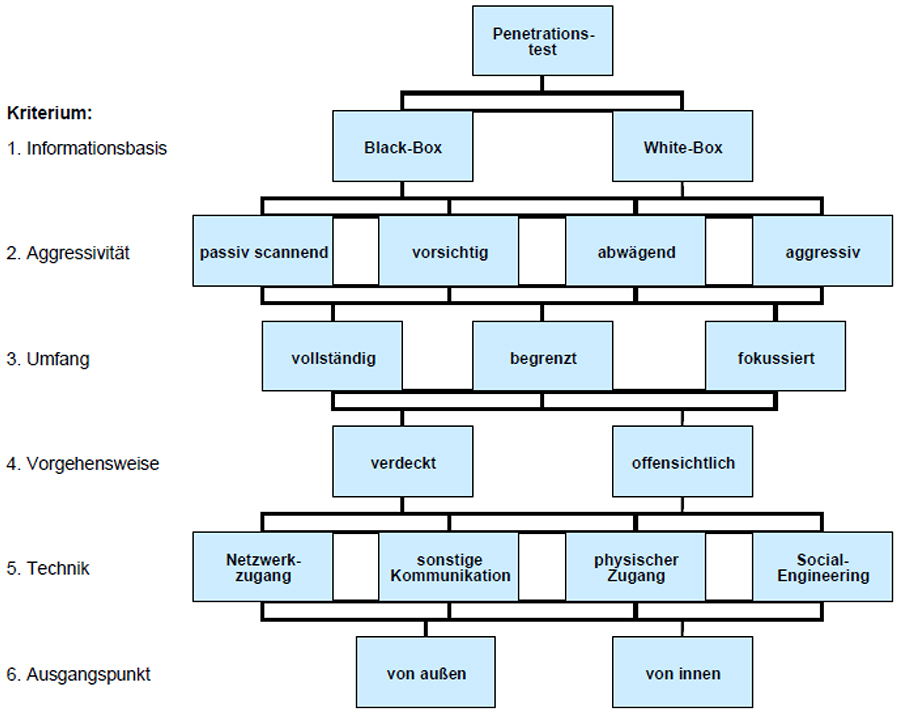
\includegraphics[scale=0.3]{bsi.jpg}
\caption{BSI Klassifikation}
\label{fig:bsi}
\end{figure}

Die Kriterien werden nachfolgend erklärt.

TODO